\documentclass[11pt,letterpaper]{article}
\usepackage[lmargin=1in,rmargin=1in,tmargin=1in,bmargin=1in]{geometry}
\usepackage{../style/homework}
\usepackage{../style/commands}
\setbool{quotetype}{false} % True: Side; False: Under
\setbool{hideans}{true} % Student: True; Instructor: False

% -------------------
% Content
% -------------------
\begin{document}

\homework{14: Due 01/13}{Geometric diagrams are to geometers what board and pieces are to chessmasters: visual aids, helpful but not indispensable.}{Richard J. Trudeau}

% Problem 1
\problem{10} Find the adjacency matrix for the graph below:
	\[
	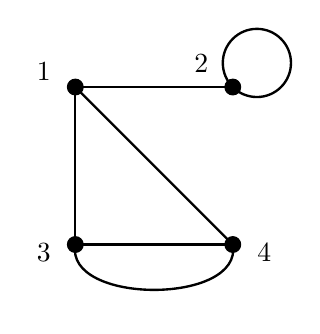
\begin{tikzpicture}
	\draw[line width=0.03cm] (2,2) -- (0,2) -- (0,0) -- (2,0);
	\draw[line width=0.03cm] (0,2) -- (2,0);
	\draw[line width=0.03cm] (0,0) to[out= -100,in= -80] (2,0);
	\draw[line width=0.03cm] (2.306,2.306) circle (0.433);
	
	\draw[fill=black] (0,0) circle (0.1);
	\draw[fill=black] (2,0) circle (0.1);
	\draw[fill=black] (0,2) circle (0.1);
	\draw[fill=black] (2,2) circle (0.1);
	
	\node at (-0.4,2.2) {$1$};
	\node at (-0.4,-0.1) {$3$};
	\node at (1.6,2.3) {$2$};
	\node at (2.4,-0.1) {$4$};
	\end{tikzpicture}
	\]



\newpage



% Problem 2
\problem{10} Find the adjacency matrix for the graph below:
	\[
	\begin{tikzpicture}
	\begin{scope}[very thick,decoration={
	markings,
	mark=at position 0.5 with {\arrow{>}}
				}
	] 
	\draw[line width=0.03cm,postaction={decorate}] (0,0) -- (0,2);
	\draw[line width=0.03cm,postaction={decorate}] (0,0) -- (2,0);
	\draw[line width=0.03cm,postaction={decorate}] (0,2) -- (2,0);
	\draw[line width=0.03cm,postaction={decorate}] (2,2) -- (0,2);	
	\draw[line width=0.03cm,postaction={decorate}] (2,0) to[out= -100,in= -80] (0,0);
	\draw[line width=0.03cm,domain= 45:225] plot ({2.306+0.433*cos(\x)}, {2.306+0.433*sin(\x)});
	\draw[line width=0.03cm,->,domain= -135:45] plot ({2.306+0.433*cos(\x)}, {2.306+0.433*sin(\x)});
	
	\draw[fill=black] (0,0) circle (0.1);
	\draw[fill=black] (2,0) circle (0.1);
	\draw[fill=black] (0,2) circle (0.1);
	\draw[fill=black] (2,2) circle (0.1);

	\end{scope}
	\end{tikzpicture}
	\]



\newpage



% Problem 3
\problem{10} Draw the graph whose adjacency matrix is given below:
	\[
	\begin{pmatrix}
	0 & 1 & 0 & 2 \\
	1 & 0 & 1 & 0 \\
	0 & 1 & 0 & 1 \\
	2 & 0 & 1 & 0 
	\end{pmatrix}
	\]



\newpage



% Problem 4
\problem{10} The adjacency matrix of a graph is given below:
	\[
	\begin{pmatrix}
	0 & 1 & 2 & 1 \\
	0 & 1 & 1 & 0 \\
	1 & 2 & 0 & 1 \\
	1 & 2 & 0 & 0 
	\end{pmatrix}
	\]

\begin{enumerate}[(a)]
\item Is the graph directed or undirected? Explain. 
\item Are there loops in the graph? Explain. 
\item How many vertices did the graph have? Explain. 
\end{enumerate}



\newpage



% Problem 5
\problem{10} Find the number of walks of length 2 from $a$ to $c$. 
	\[
	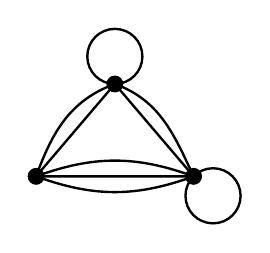
\begin{tikzpicture}
	\draw[line width=0.03cm] (0,0) -- (2,0) -- (1,1.1732) -- (0,0);
	\draw[line width=0.03cm] (0,0) to[out= -20,in= -160] (2,0);
	\draw[line width=0.03cm] (2,0) to[out= 115,in= -20] (1,1.1732);
	\draw[line width=0.03cm] (1,1.1732) to[out= 200,in= 70] (0,0);
	\draw[line width=0.03cm] (0,0) to[out= 20,in= 160] (2,0);
	\draw[line width=0.03cm] (1,1.5232) circle (0.35);
	\draw[line width=0.03cm] (2.247,-0.247) circle (0.35);

	\draw[fill=black] (0,0) circle (0.1);
	\draw[fill=black] (1,1.1732) circle (0.1);
	\draw[fill=black] (2,0) circle (0.1);
	\end{tikzpicture}
	\]


\end{document}